\documentclass[10pt]{article}
\usepackage[margin=1in]{geometry}
\usepackage{booktabs}
\usepackage{graphicx}
\usepackage{xcolor}
\usepackage{amsmath}
\usepackage{array}
\usepackage[hidelinks]{hyperref}
\usepackage{enumitem}

\definecolor{good}{HTML}{1E8449}
\definecolor{bad}{HTML}{B03A2E}
\definecolor{neut}{HTML}{6E7F8D}
\newcommand{\grsup}{\textcolor{good}{\textbf{supported}}}
\newcommand{\fals}{\textcolor{bad}{\textbf{falsified}}}
\newcommand{\under}{\textcolor{neut}{\textbf{underpowered}}}
\newcommand{\nom}{\textcolor{neut}{\textbf{nomination}}}
\newcommand{\gene}[1]{\textit{#1}}
\newcommand{\code}[1]{\texttt{\small #1}}
\graphicspath{{figures_osd462/}}

\title{\textbf{Six-Recommendation Integration:\\
Cross-Omic Decoupling of the Spaceflight Kidney DCT/NCC Phenotype}}
\author{RRRM-2 Kidney Transcriptome project --- consolidated results addendum}
\date{2026-05-22}

\begin{document}
\maketitle

\noindent
This addendum reports the six analytical recommendations of the May 2026 strategy
memo, run end-to-end and integrated into the v10 phenotype-anchored frame. The
guiding thesis is unchanged and is the one the memo endorses: \emph{the established
spaceflight DCT/NCC phenotype sits inside a recurrent kidney-wide RNA remodeling
context that is cross-omically decoupled --- it recurs in transcriptomes, fails as
a protein-abundance story, and resolves at the NCC/SPAK regulatory-phosphorylation
layer.} Each recommendation is graded conservatively. Numbers are drawn from the
run artifacts \code{run\_20260522\_osd462\_anchor}, \code{run\_20260522\_regulator\_activity},
\code{run\_20260522\_phenotype\_anchor}, \code{run\_20260522\_celltype\_decomposition},
and \code{run\_20260522\_physiology\_assessment}.

\begin{figure}[t]
\centering
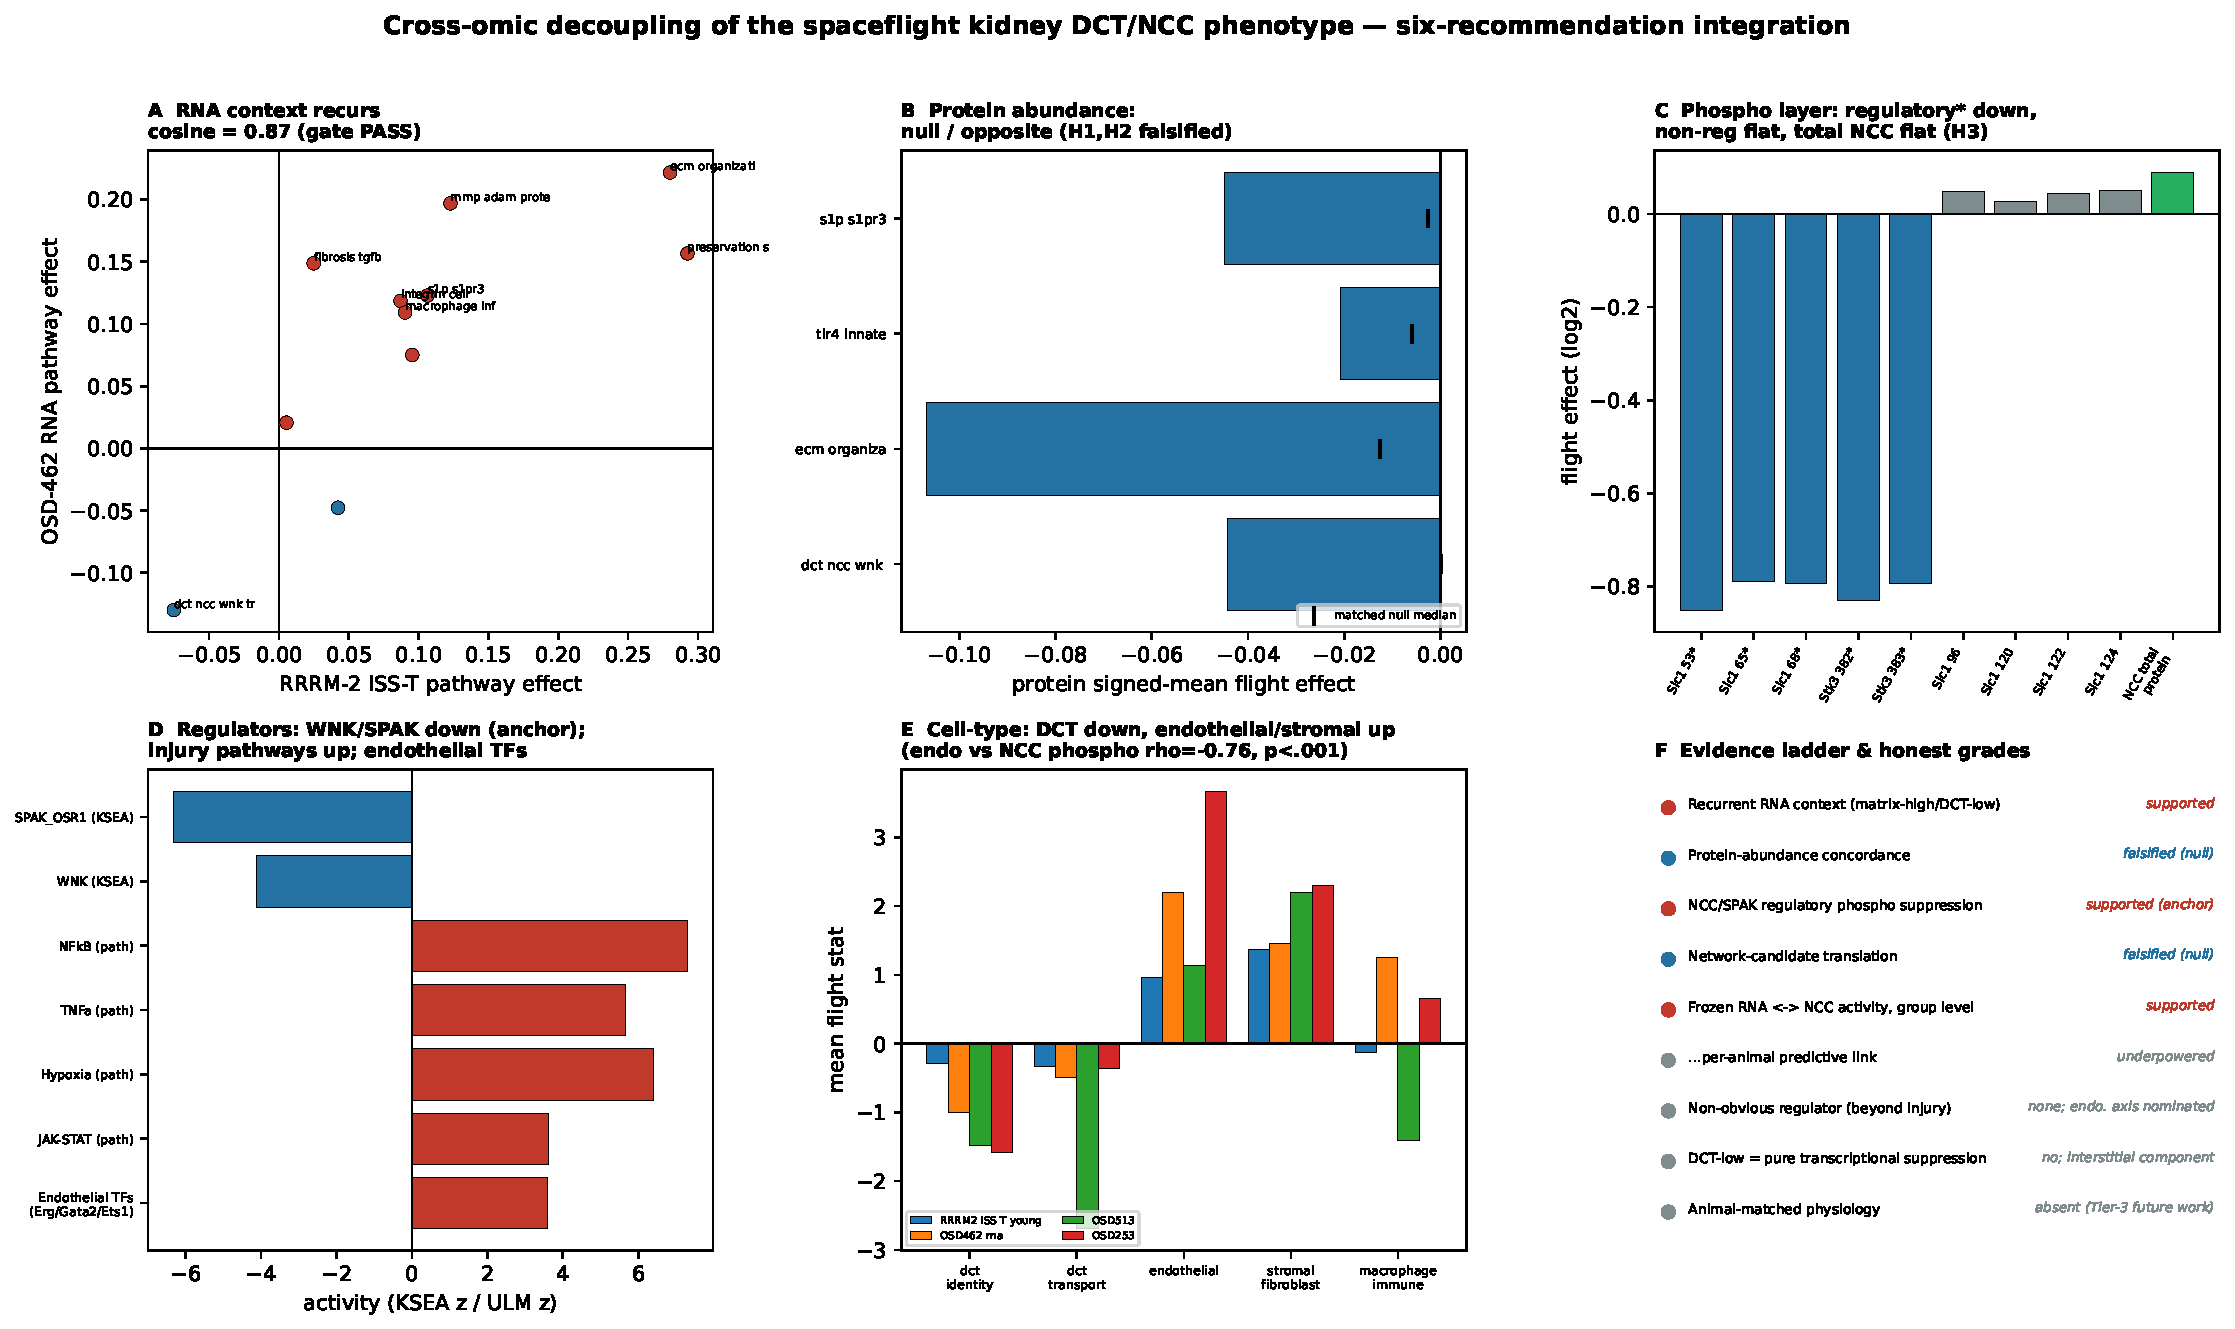
\includegraphics[width=\textwidth]{fig_sixrec_integration.pdf}
\caption{\textbf{Consolidated six-recommendation integration.}
(A) The matrix-high/DCT-low RNA pathway vector recurs between RRRM-2 ISS-T and
OSD-462 (cosine $=0.87$, gate PASS).
(B) Matched-null protein-abundance concordance is null/opposite for both matrix
(ECM) and DCT families (H1, H2 falsified).
(C) On the WNK--SPAK/OSR1--NCC chain, activating regulatory phosphosites (asterisk)
are strongly suppressed while non-regulatory \gene{Slc12a3} sites and total NCC
protein are flat (H3 supported).
(D) KSEA returns WNK and SPAK/OSR1 inferred-activity down (anchor); decoupler
recurrent pathway activity is dominated by expected injury programs, with an
endothelial/vascular TF module as the most coherent non-obvious recurrent signal.
(E) Marker-panel decomposition: DCT identity \emph{and} transport fall while
endothelial/stromal compartments rise across cohorts; per animal the endothelial
score anti-correlates with NCC regulatory phospho ($\rho=-0.76$, $p<0.001$).
(F) Evidence ladder and honest grades.}
\label{fig:sixrec}
\end{figure}

\section*{Recommendation 3 --- Cross-omic transcript$\rightarrow$protein$\rightarrow$phospho dissociation \quad[\grsup\ as the central result]}
The OSD-462 / RR-10 anchor resolves the memo's central claim. (i)~\textbf{RNA recurrence:}
the matrix-high/DCT-low pathway vector recurs between RRRM-2 ISS-T and OSD-462 RNA
(cosine $=0.869$, bootstrap CI $[0.65, 0.90]$, leave-one-pathway-out range
$0.82$--$0.90$; 11 shared pathways) --- \textbf{gate PASS}. (ii)~\textbf{Protein
abundance does not mirror RNA:} the genome-wide RNA$\leftrightarrow$protein
flight-effect Spearman is $0.043$; the ECM family signed-mean protein effect is
$-0.107$ (\emph{opposite} to the RNA-predicted increase; cross-study concordance
$-0.40$) and the DCT family is null ($-0.044$); no targeted set is concordant in
its predicted direction (\textbf{H1, H2 falsified}). (iii)~\textbf{Phospho layer:}
total NCC protein is flat ($+0.089$), yet the NCC N-terminal activating cluster
(mean $-0.83$) and SPAK/OSR1 sites (mean $-0.41$) are strongly suppressed --- 7
NCC-regulatory and 3 SPAK/OSR1 sites significant-down, non-regulatory \gene{Slc12a3}
sites flat (\textbf{H3 supported}). (iv)~\textbf{Network translation:} RRRM-2
network-candidate genes are \emph{not} enriched among protein- or phospho-changing
genes ($p_{\min}=0.23$/$0.25$; \textbf{H4 falsified}). The transporter lesion is a
post-translational/activity event embedded in an RNA context, not a protein-abundance
signature.

\section*{Recommendation 1 --- Frozen RNA predictor / phenotype anchor \quad[group \grsup; per-animal \under]}
A phosphoproteomics-naive DCT/NCC-WNK transport RNA score and a pre-specified NCC
regulatory-phospho activity score (\gene{Slc12a3} T53/58/65/68, \gene{Stk39}
S382/383) were matched across 20 RR-10 animals. \textbf{Group level (concordant):}
flight lowers both the RNA program ($-0.324$) and NCC regulatory phosphorylation
($-1.298$); the regulatory cluster is suppressed $\sim$4.3$\times$ more than
non-regulatory NCC sites ($-1.30$ vs $-0.30$). \textbf{Per animal:} the link is
positive but not significant (Spearman $+0.328$, $p=0.16$; condition-adjusted
$+0.365$, $p=0.11$) --- the anticipated underpowered-at-$n{=}20$ outcome.
\textbf{Controls:} dropping the \gene{Slc12a3} transcript preserves the group
concordance ($-0.247$); but non-regulatory NCC phosphosites \emph{also} covary
per-animal with the RNA score ($+0.555$, $p=0.011$), so per-animal specificity is
\emph{not} exclusive to regulatory sites. The honest claim ceiling is therefore
group-level concordance with magnitude specificity, not a validated per-animal
predictor; reported as such.

\section*{Recommendation 2 --- Search for a non-obvious regulator \quad[KSEA anchor \grsup; Layer B \nom]}
\textbf{Layer A (KSEA, OSD-462 phosphoproteome):} the WNK--SPAK/OSR1 positive
control passes --- SPAK/OSR1 $z=-6.31$ ($p=2.8\times10^{-10}$), WNK $z=-4.12$
($p=3.7\times10^{-5}$), both inferred-activity-down --- certifying the
activity-inference machinery. \textbf{Layer B (decoupler ULM; PROGENy + CollecTRI,
mouse):} run within each of five cohorts (RRRM-2 ISS-T, RRRM-2 LAR, OSD-462,
OSD-513, OSD-253), never by pooling. Across the four terminal-flight cohorts the
recurrently-up pathways are the \emph{expected} injury/inflammation programs
(NF-$\kappa$B, TNF$\alpha$, JAK-STAT, Hypoxia) --- all of which \emph{reverse sign}
in the RRRM-2 LAR live-return arm, consistent with recovery. Of 751 scored TFs,
none recur as inferred-down; the most coherent non-obvious recurrent signal is an
\textbf{endothelial/vascular TF module (\gene{Erg}, \gene{Gata2}, \gene{Ets1})},
consistent with the S1P/S1PR3 and adhesion components of the RNA neighborhood, with
\gene{Spi1} (macrophage) and retinoid receptors (\gene{Rara}/\gene{Rarg}) also
recurrent. \textbf{Verdict (claim discipline):} no single non-obvious upstream
driver dominates beyond known injury/stress pathways; the endothelial/vascular axis
is nominated as a candidate context axis, not a proven regulator.

\section*{Recommendation 4 --- Cell-type / spatial evidence \quad[bounds interpretation]}
A curated marker-panel decomposition separates DCT \emph{identity} (\gene{Pvalb},
\gene{Trpm6}, \gene{Calb1}, \ldots) from the DCT \emph{transport} program. Across
the four flight cohorts, \emph{both} DCT identity (OSD-462 $-1.00$, OSD-513 $-1.48$,
OSD-253 $-1.59$) and DCT transport fall, while endothelial (OSD-462 $+2.20$) and
stromal/fibroblast (OSD-462 $+1.45$) compartments rise recurrently. In OSD-462 the
per-sample endothelial ($+1.00$, $p=0.036$) and stromal ($+0.67$, $p=0.054$) flight
increases are the strongest moves, and \textbf{per animal the endothelial score
anti-correlates with NCC regulatory phospho ($\rho=-0.76$, $p=0.0004$)}; stromal
likewise ($\rho=-0.51$, $p=0.023$). Because DCT identity falls alongside transport
and interstitial compartments expand, the bulk DCT-low signal carries a genuine
composition / interstitial-expansion component and \emph{cannot} be read as pure
cell-autonomous transcriptional suppression. This is precisely why the
regulatory-phosphosite layer --- normalized within the phosphoproteome and
$\sim$4$\times$ more suppressed at regulatory than non-regulatory sites --- is the
more reliable transporter readout. Cell-type analysis here \emph{bounds}
interpretation and reinforces the cross-omic decoupling thesis rather than
overturning it.

\section*{Recommendation 5 --- Physiology \quad[absent in-cohort; Tier-2/3 literature ladder]}
The OSD-462 record contains only molecular assays; no urine/serum electrolyte,
blood-pressure, or per-animal kidney-function endpoint is present, so no
animal-level physiology$\leftrightarrow$RNA inference is possible. The same-mission
Cosmic Kidney Disease study (Siew et al.\ 2024) supplies a \textbf{Tier-2
morphology anchor}: flight reduces DCT NCC-positive (tNCC) density by $47.6\%$
($p=0.001$; total area $-26.3\%$, $p=0.082$; mean object area $+34.1\%$,
$p=0.028$), a morphological correlate consistent with the measured NCC/SPAK
phospho suppression. Group-level plasma and urine electrolytes (Na, Cl, Ca, Mg, K,
PO$_4$) and fractional-excretion readouts exist in that study but cannot be
matched to the OSD-462 omics animals. Per the memo: state the absence explicitly;
animal-matched electrolyte/blood-pressure endpoints remain Tier-3 future work.

\section*{Recommendation 6 --- Kill weak branches (main vs supplement triage)}
Table~\ref{tab:triage} is the placement decision derived from the current evidence
grades. The ruthless main-text spine is: (1)~prior work established the DCT/NCC
phenotype; (2)~a DCT/NCC-low RNA context recurs across RRRM-2, OSD-513, OSD-462;
(3)~that context is matrix/adhesion/proteolysis/S1P/innate/stress-up,
DCT/NCC-WNK-down; (4)~protein abundance does not mirror it; (5)~NCC/SPAK
phosphoproteomics + KSEA locate the transporter phenotype at the activity layer;
(6)~animal-matched analysis supports group-level concordance, not per-animal
prediction; (7)~marker panels show an interstitial-expansion component bounding the
"state" language; (8)~regulator, network, age, and LAR analyses define boundaries
and a single nominated endothelial context axis.

\begin{table}[t]
\centering\small
\renewcommand{\arraystretch}{1.15}
\begin{tabular}{p{6.4cm} l p{4.6cm}}
\toprule
\textbf{Component} & \textbf{Placement} & \textbf{Grade / reason}\\
\midrule
Cross-cohort RNA recurrence (matrix-high/DCT-low) & main & \grsup\ (cosine 0.87)\\
OSD-462 protein-abundance concordance & main & \fals\ --- the punchline\\
NCC/SPAK regulatory phospho + KSEA & main & \grsup\ (Tier-1 anchor)\\
Phenotype-anchor (animal-matched RNA$\leftrightarrow$NCC) & main (careful) & group \grsup, per-animal \under\\
Cell-type marker-panel decomposition & main (short) & bounds interpretation\\
Regulator Layer B (TF/pathway recurrence) & main-short / supp.\ & \nom\ (endothelial axis)\\
Physiology ladder (Siew tNCC morphometry) & discussion & Tier-2 literature anchor\\
Network-candidate translation (Layer 3) & supplement & \fals\ (neg.\ method)\\
Age-rewiring failure & supplement + boundary & not supported (history)\\
LAR attenuation/divergence & supplement & context (recovery reversal)\\
OSD-253 / TLR4 & supplement & association, not pillar\\
WGCNA grey60 & supplement & annotation\\
LIONESS / node2vec & supplement & \fals\ (neg.\ method)\\
External aging projection & supplement & rules out aging mimicry\\
\bottomrule
\end{tabular}
\caption{Main-text vs supplement triage (memo Rec 6), graded from the current results.}
\label{tab:triage}
\end{table}

\section*{Consolidated evidence grades}
\begin{table}[h]
\centering\small
\renewcommand{\arraystretch}{1.2}
\begin{tabular}{p{8.6cm} l}
\toprule
\textbf{Claim} & \textbf{Grade}\\
\midrule
Matrix-high/DCT-low RNA context recurs across cohorts & \grsup\\
RNA recurrence translates to matrix/transporter protein abundance & \fals\\
NCC/SPAK regulatory-phosphorylation suppression (activity layer) & \grsup\ (anchor)\\
Network-candidate genes translate to protein/phospho changes & \fals\\
Frozen RNA score tracks NCC activity --- group level & \grsup\\
Frozen RNA score predicts NCC activity --- per animal & \under\\
A non-obvious upstream regulator beyond injury programs & \nom\ (endothelial axis only)\\
Bulk DCT-low is pure DCT transcriptional suppression & \textcolor{neut}{\textbf{no}} (interstitial component)\\
Animal-matched physiology endpoint & \textcolor{neut}{\textbf{absent}} (Tier-3 future work)\\
\bottomrule
\end{tabular}
\caption{Honest claim grades after running all six recommendations.}
\end{table}

\noindent\textbf{What this paper claims / does not claim.} It contributes a
reproducible, cross-omically decoupled RNA context map around an \emph{established}
phenotype, with explicit null boundaries (protein abundance, network translation),
an interstitial-expansion caveat on the bulk DCT signal, and a single nominated
endothelial/vascular context axis. It does \emph{not} discover NCC dephosphorylation
(Siew et al.\ 2024), prove a causal driver, claim a validated per-animal predictor,
or establish physiology without direct endpoints.

\end{document}
